\documentclass[UTF8,a4paper,11pt,fontset=none]{ctexart}

\usepackage{geometry}
\usepackage{graphicx}
\usepackage{booktabs}
\usepackage{float}
\usepackage{hyperref}
\usepackage{amsmath}
\usepackage{xcolor}
\usepackage{caption}

\setCJKmainfont{Songti SC}
\setCJKsansfont{Heiti SC}
\setCJKmonofont{Hiragino Sans GB}

\geometry{left=2.4cm,right=2.4cm,top=2.3cm,bottom=2.3cm}
\hypersetup{
  colorlinks=true,
  linkcolor=blue,
  urlcolor=blue
}
\captionsetup{font=small,labelfont=bf}

\title{HW1：基于 NumPy 从零构建三层神经网络分类器\\实现地表覆盖图像分类}
\author{姓名：\underline{\hspace{4cm}} \quad 学号：\underline{\hspace{4cm}}}
\date{\today}

\begin{document}
\maketitle

\begin{abstract}
本文基于 EuroSAT\_RGB 遥感图像数据集，实现了一个不依赖 PyTorch、TensorFlow 或 JAX 的多层感知机分类器。模型的前向传播、反向传播、Softmax 交叉熵损失、L2 正则化、随机梯度下降、动量项以及学习率衰减均使用 NumPy 手动实现。实验采用分层划分方式构造训练集、验证集和测试集，并通过验证集准确率保存最优模型权重。最终最佳模型在测试集上取得了 68.27\% 的分类准确率。本文同时给出了训练曲线、混淆矩阵、第一层权重可视化和错误样例分析。
\end{abstract}

\section{任务描述}

本次作业要求手工搭建一个三层神经网络分类器，在 EuroSAT\_RGB 数据集上完成地表覆盖图像分类任务。EuroSAT\_RGB 包含 10 个类别，分别为 AnnualCrop、Forest、HerbaceousVegetation、Highway、Industrial、Pasture、PermanentCrop、Residential、River 和 SeaLake。每张图像为 RGB 遥感图像，原始大小为 $64\times64$。

本实验严格遵守作业要求：不使用 PyTorch、TensorFlow、JAX 等自动微分深度学习框架，仅使用 NumPy 完成矩阵运算和梯度计算。代码文件为 \texttt{src/train\_numpy\_mlp.py}，生成报告所用的图像位于 \texttt{outputs/} 目录下。

\section{数据处理}

为了降低全连接网络的输入维度和训练开销，实验将所有图像缩放为 $32\times32$ 的 RGB 图像，然后展平成长度为 $32\times32\times3=3072$ 的向量。像素值先归一化到 $[0,1]$，再使用训练集均值和标准差进行标准化。数据集采用固定随机种子进行分层划分，保证每个类别在训练集、验证集和测试集中的比例一致。

\begin{table}[H]
  \centering
  \caption{数据集划分}
  \begin{tabular}{lc}
    \toprule
    数据子集 & 样本数量 \\
    \midrule
    训练集 & 18900 \\
    验证集 & 4050 \\
    测试集 & 4050 \\
    \bottomrule
  \end{tabular}
\end{table}

\section{模型结构与训练方法}

模型采用三层全连接神经网络结构，即输入层、两个隐藏层和一个 Softmax 输出层。设输入样本为 $x$，网络前向传播形式为：
\begin{align}
  h_1 &= f(xW_1+b_1),\\
  h_2 &= f(h_1W_2+b_2),\\
  o &= h_2W_3+b_3,\\
  p_i &= \frac{\exp(o_i)}{\sum_j \exp(o_j)}.
\end{align}

其中 $f(\cdot)$ 为隐藏层激活函数，本实验对 ReLU 和 Tanh 进行了比较。损失函数采用 Softmax 交叉熵，并加入 L2 正则化：
\begin{equation}
  \mathcal{L}=-\frac{1}{N}\sum_{n=1}^{N}\log p_{n,y_n}
  + \frac{\lambda}{2}\sum_l \lVert W_l\rVert_2^2.
\end{equation}

训练过程使用小批量随机梯度下降，并在部分配置中加入 momentum 动量项以改善优化稳定性。每轮训练后在验证集上评估准确率，并保存验证集准确率最高的模型参数。学习率采用指数衰减策略：
\begin{equation}
  \eta_t = \eta_0 \gamma^t,
\end{equation}
其中 $\eta_0$ 为初始学习率，$\gamma$ 为衰减系数。

\section{超参数搜索}

实验比较了不同隐藏层规模、激活函数、学习率、学习率衰减、L2 正则化强度和 momentum。由于本作业重点是从零实现反向传播和优化过程，超参数搜索规模保持较小，以便在普通 CPU 环境中可复现。

\begin{table}[H]
  \centering
  \caption{超参数搜索结果}
  \small
  \begin{tabular}{cccccccc}
    \toprule
    实验编号 & 隐藏层维度 & 激活函数 & 初始学习率 & 学习率衰减 & L2 正则化 & 动量 & 最优验证准确率 \\
    \midrule
    1 & [384, 96] & ReLU & 0.010 & 0.97 & $1\times10^{-3}$ & 0.9 & 67.68\% \\
    2 & [256, 64] & ReLU & 0.012 & 0.97 & $1\times10^{-3}$ & 0.9 & 67.33\% \\
    3 & [256, 64] & ReLU & 0.012 & 0.97 & $7\times10^{-4}$ & 0.9 & 67.01\% \\
    4 & [256, 64] & ReLU & 0.035 & 0.95 & $7\times10^{-4}$ & 0.0 & 66.91\% \\
    5 & [256, 128] & Tanh & 0.015 & 0.95 & $1\times10^{-4}$ & 0.0 & 58.59\% \\
    \bottomrule
  \end{tabular}
\end{table}

最佳配置为实验 1：隐藏层维度为 $[384,96]$，激活函数为 ReLU，初始学习率为 0.010，学习率衰减系数为 0.97，L2 正则化强度为 $1\times10^{-3}$，momentum 为 0.9。相比不使用动量的配置，momentum 能在较小学习率下更快进入高准确率区域；同时较强的 L2 正则化缓解了动量训练后期训练准确率较高带来的过拟合风险。Tanh 对照组收敛较慢，最终准确率明显低于 ReLU。

\section{训练曲线与测试结果}

图 \ref{fig:curves} 展示了最佳模型在训练过程中的交叉熵损失和准确率变化。可以看到，训练损失整体随训练轮数下降，训练准确率持续上升；验证准确率在第 73 轮附近达到最高。由于模型为全连接网络，且输入图像被展平，模型缺少卷积网络中的局部平移不变性，因此整体准确率仍然有限。

\begin{figure}[H]
  \centering
  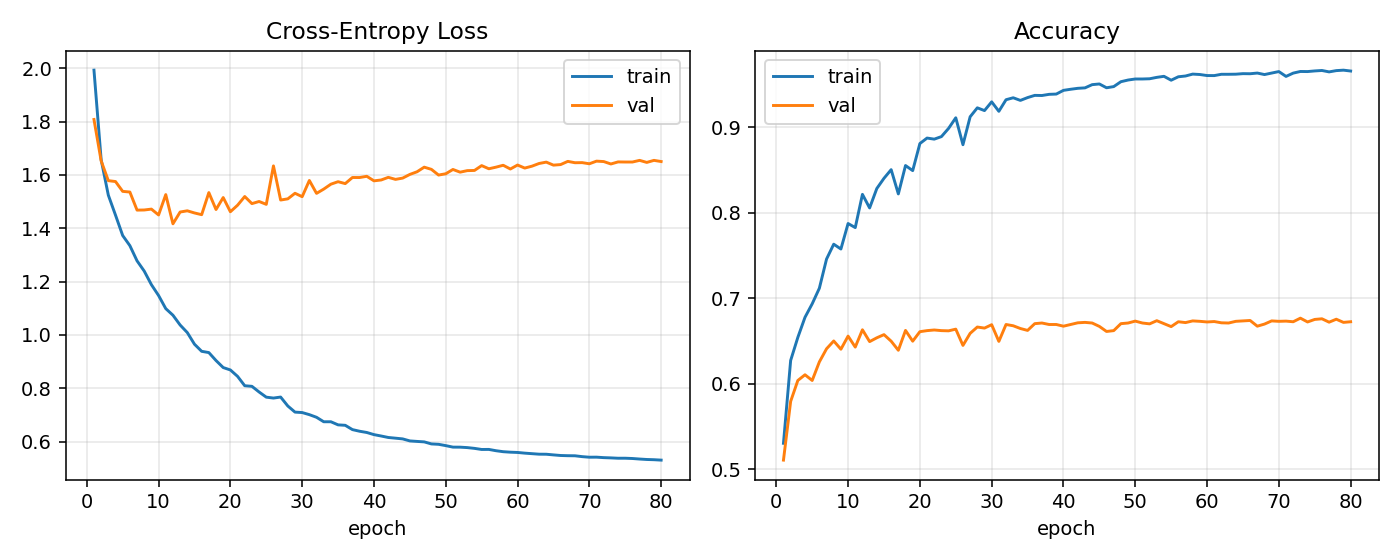
\includegraphics[width=0.95\linewidth]{outputs/learning_curves.png}
  \caption{训练集与验证集上的损失曲线和准确率曲线}
  \label{fig:curves}
\end{figure}

使用验证集上保存的最佳权重，在测试集上得到的准确率为 68.27\%。图 \ref{fig:confusion} 给出了测试集混淆矩阵。从混淆矩阵可以看出，Forest、Industrial 和 SeaLake 等类别识别相对较好；而 AnnualCrop、PermanentCrop、Pasture、HerbaceousVegetation 之间更容易混淆，这些类别在颜色和纹理上具有较高相似性。

\begin{figure}[H]
  \centering
  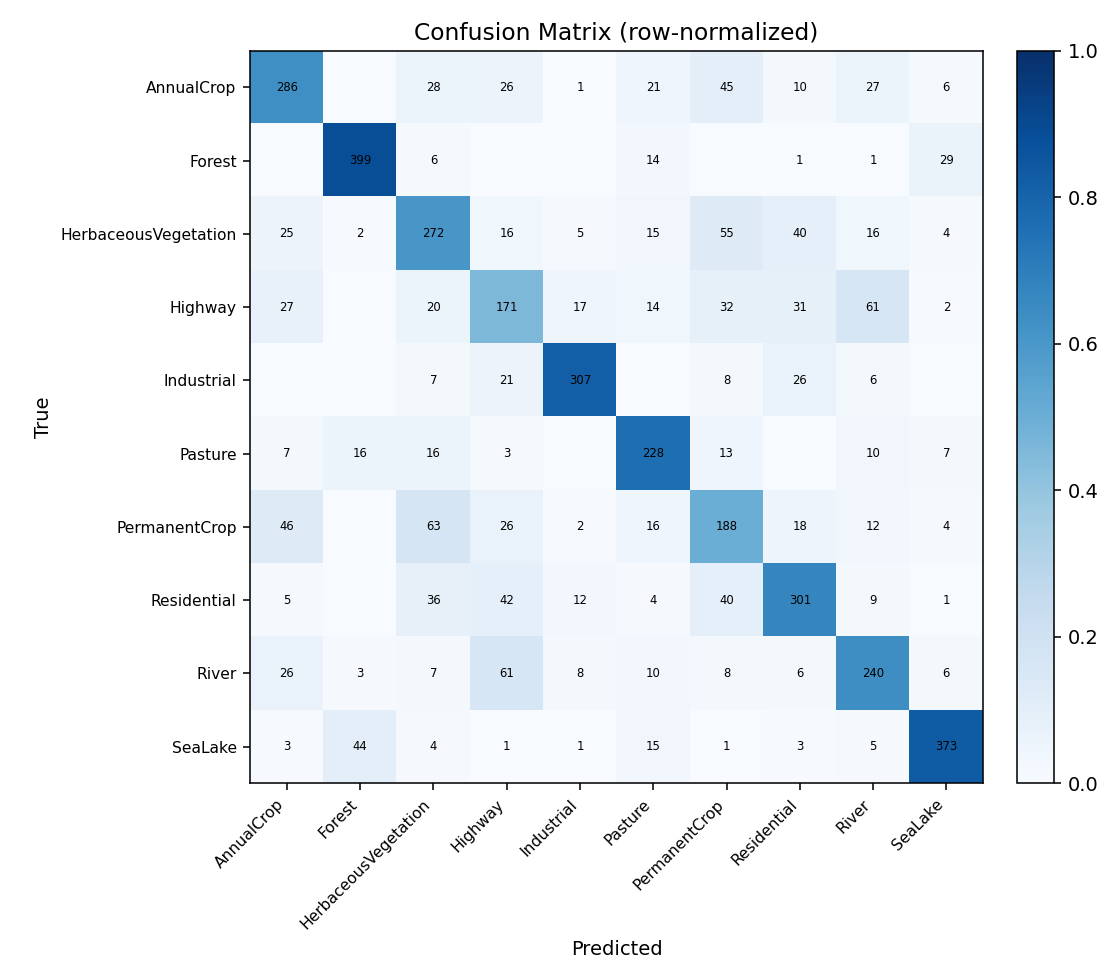
\includegraphics[width=0.82\linewidth]{outputs/confusion_matrix.png}
  \caption{测试集混淆矩阵}
  \label{fig:confusion}
\end{figure}

\section{第一层权重可视化}

为了观察模型是否学习到空间或颜色模式，将第一层隐藏层权重重新恢复为 $32\times32\times3$ 的图像形式，并选择范数较大的若干隐藏单元进行可视化，如图 \ref{fig:weights} 所示。由于 MLP 直接处理展平后的像素向量，第一层权重主要表现为较粗粒度的颜色和低频空间响应，而不是卷积网络中常见的局部边缘滤波器。这说明模型能够捕捉一定的植被、水体、土壤和城市区域颜色倾向，但对局部结构的建模能力较弱。

\begin{figure}[H]
  \centering
  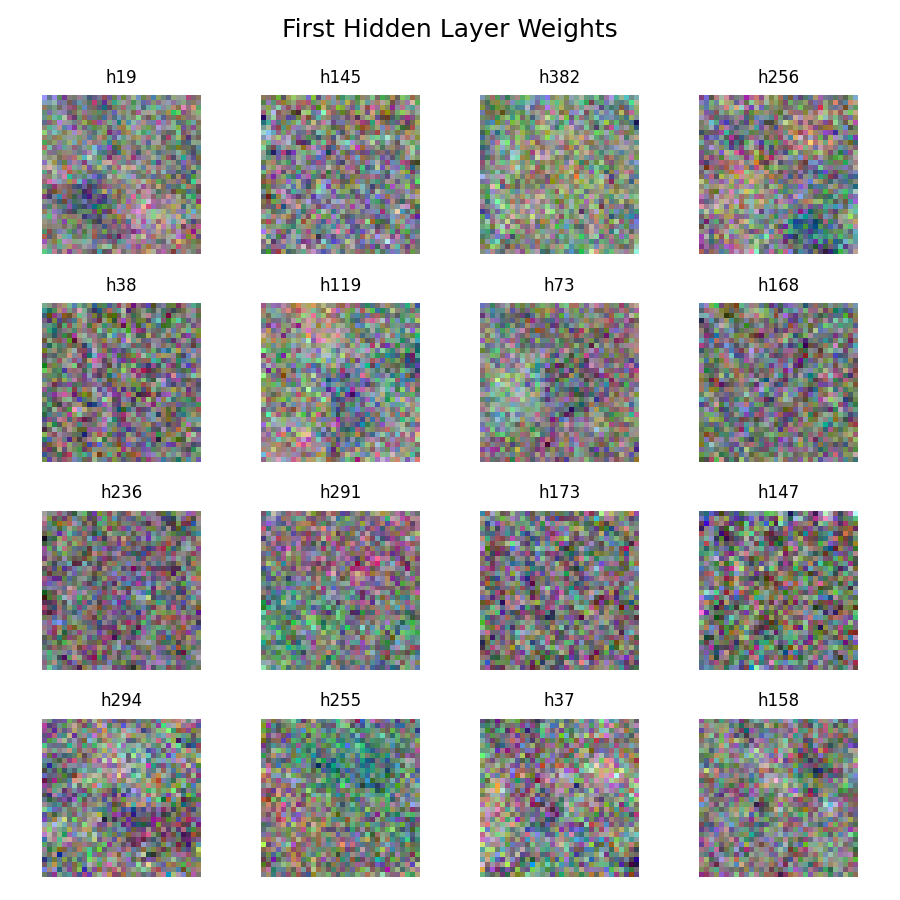
\includegraphics[width=0.75\linewidth]{outputs/first_layer_weights.png}
  \caption{第一层隐藏层权重可视化}
  \label{fig:weights}
\end{figure}

\section{错误分析}

图 \ref{fig:errors} 展示了测试集中若干分类错误样例。可以观察到，Highway 和 River 常出现混淆，因为二者在遥感图像中都可能呈现细长、连续的线状结构。AnnualCrop、PermanentCrop、Pasture 和 HerbaceousVegetation 之间也较容易混淆，因为这些类别通常具有相近的绿色或棕色纹理，并且在低分辨率图像中边界和几何形状并不总是清晰。

\begin{figure}[H]
  \centering
  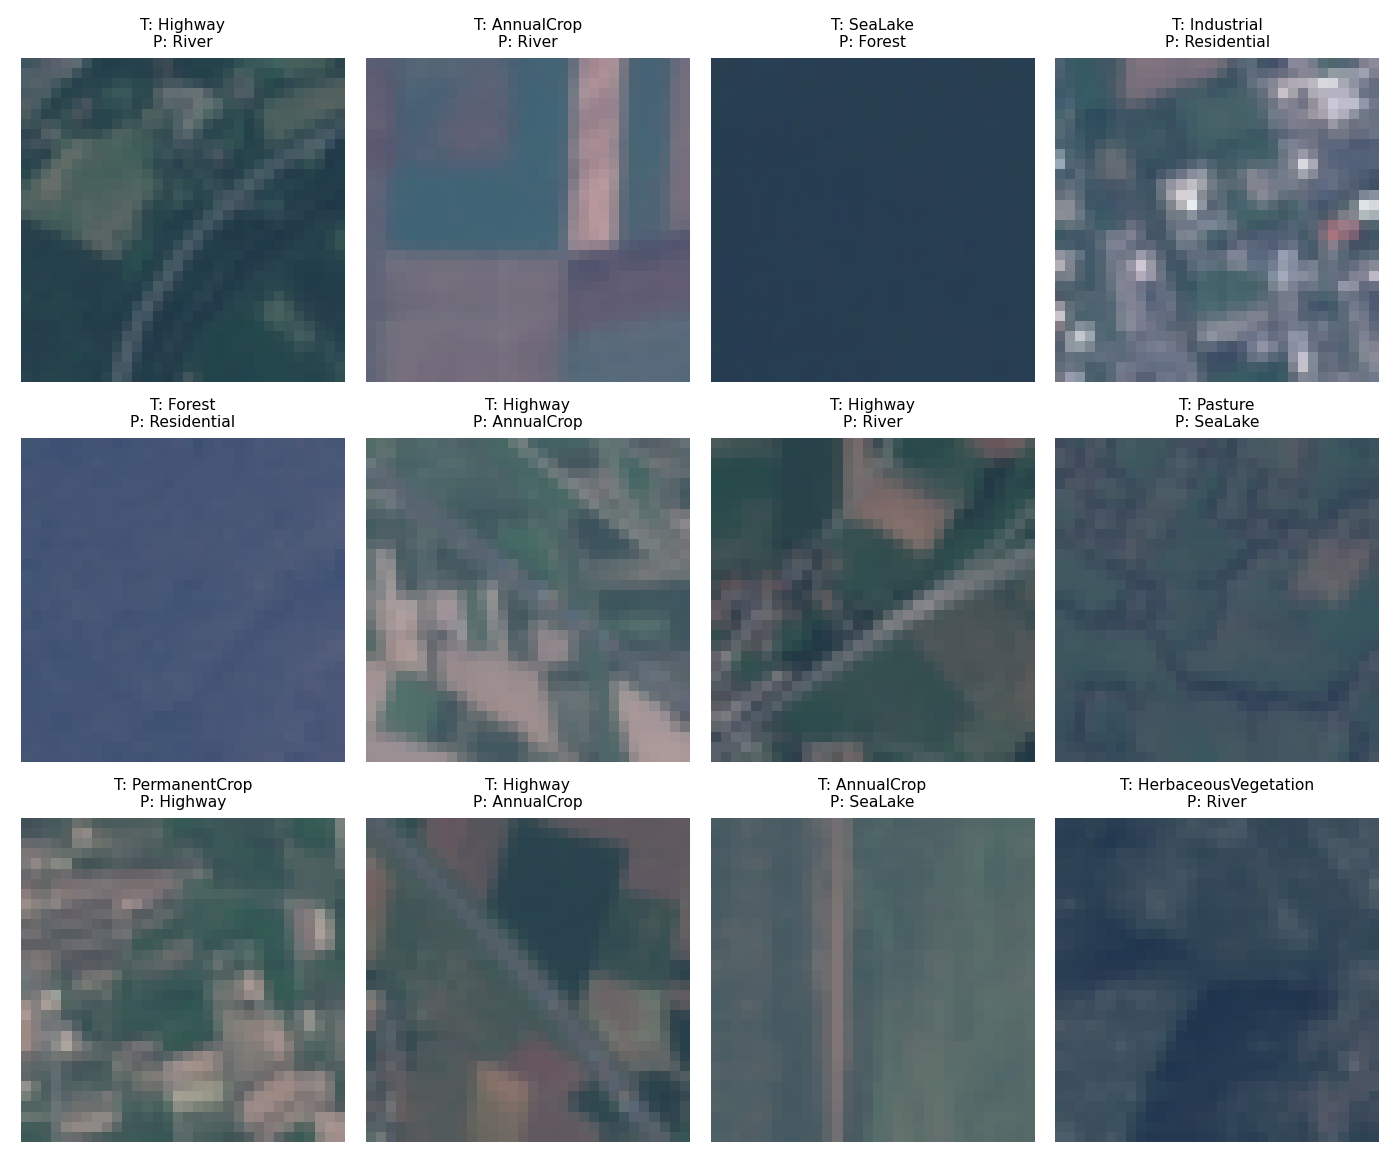
\includegraphics[width=0.95\linewidth]{outputs/error_examples.png}
  \caption{测试集分类错误样例}
  \label{fig:errors}
\end{figure}

总体来看，错误主要来自两方面。第一，遥感场景类别本身存在视觉相似性，例如农田、牧场和草地的光谱与纹理特征相近；第二，MLP 缺少显式的空间局部建模能力，图像展平后相邻像素关系没有被结构化利用。因此，若允许使用卷积神经网络，预期可以进一步提升分类性能。但本实验的重点在于手工实现自动微分以外的神经网络训练流程，当前结果能够反映 MLP 在该任务上的基本能力和局限。

\section{复现说明与提交链接}

在作业目录下运行以下命令可以复现实验：

\begin{verbatim}
python3 src/train_numpy_mlp.py --data-dir EuroSAT_RGB --out-dir outputs --search
\end{verbatim}

运行以下命令可以编译本文的 LaTeX 报告：

\begin{verbatim}
xelatex report_hw1.tex
\end{verbatim}

模型权重已保存为：
\begin{verbatim}
outputs/best_model.npz
\end{verbatim}

作业要求的公开仓库和模型下载链接如下。

\begin{table}[H]
  \centering
  \caption{提交链接}
  \begin{tabular}{ll}
    \toprule
    项目 & 链接 \\
    \midrule
    Public GitHub Repo & \url{https://github.com/huang200309/eurosat-numpy-mlp-hw1} \\
    模型权重下载地址 & \url{https://github.com/huang200309/eurosat-numpy-mlp-hw1/raw/main/outputs/best_model.npz} \\
    \bottomrule
  \end{tabular}
\end{table}

\end{document}
